%% utexasthesis.cls is available from https://github.com/linguistics/utexas-latex
\documentclass{utexasthesis}
% \documentclass[copyright,12pt,onehalfspacing,draft]{utexasthesis}

%% Required fields
%% ===============
%% Full official title of your thesis (use \\ to force a line break)
\title{Computer Vision for Radar Interferometry \\ Over West Texas }
%% Your full official name
\author{Scott Staniewicz}
%% Month and year of graduation (month may be May, August, or December)
\graduationdate{May}{2022}
%% Your thesis supervisor, full name only
\supervisor{Jingyi Ann Chen}
%% Your thesis co-supervisor, if any (leave commented if not applicable)
% \cosupervisor{Cosupervisor Name}
%% Other committee members full names, comma-separated.
%% Comment this out if empty, e.g., for a masters thesis with only a supervisor and cosupervisor.
\othercommitteemembers{Srinivas Bettadpur, Todd Humphreys, Jon Olson, Peter Hennings}

%% Optional customizations
%% =======================
%% Use Palatino as the primary font face
\usepackage{palatino}
\usepackage{amsmath}
\usepackage{bm}
\usepackage{minted}
\usepackage{epsfig}
%% and Computer Modern Typewriter Proportional as the teletype font face
\renewcommand*\ttdefault{cmvtt}

\begin{document}

%% This produces the copyright page (if specified), the signature page, and title page.
\maketitle

%% The dedication is optional and fills an entire page.
\begin{dedication}
  I dedicate this to Moxie
\end{dedication}

%% The acknowledgments, abstract, and table(s) of contents/tables/figures pages are numbered with roman numerals.

%% The acknowledgments is optional and fills an entire page.
\begin{acknowledgments}
  Many thanks to Moxie
\end{acknowledgments}

%% The abstract is required.
\begin{abstract}
  Indent and begin abstract here. It should be a concise statement of the nature and content of the ETD. The text must be either double-spaced or 1.5-spaced. Abstracts should be limited to 350 words.
\end{abstract}

%% The table of contents is required.
\maketableofcontents

%% The following pages are numbered with arabic numerals, starting with 1

\chapter{Introduction}

Your ETD must be correct in spelling and punctuation and presented in a consistent, structured format. A single, legible font must be used throughout, the only exceptions being in tables, figures, graphs, appendices, and supplemental files. Headings may be bolded and no more than 2 points larger than the rest of the text. The font size should be sufficient for the average person to read the document on a computer monitor without difficulty (12-pt is recommended.) Accuracy and consistency in presentation and form make your ETD a usable research tool for other readers.


\section{A Section}

This is the first line of the first section of the first chapter, but not the first line of the first chapter, which belongs to no section.

\chapter{InSAR Background}

\section{SAR Basics}

\subsection{SAR Constellations}

- Make a figure with historial sar mission, and include private sector companies as well

\url{https://digitalcommons.usu.edu/cgi/viewcontent.cgi?article=5092&context=smallsat}

\url{https://www.newspace.im/ }

\url{https://www.newspace.im/constellations/iceye}


- There may be more SAR satellites launched in the next 5 years than cumulatively before this

\section{InSAR}

\section{InSAR Time Series}

stacking for avg rate

SBAS linear system. doesn't need to be short baseline. just a way to solve for the phase at each date

Phase linking approaches solve for this using an eptimization on each pixels time-covariance matrix.

\subsection{Uncertainty}

Several ways for uncertainty.

jackknife (maybe look into the NSBAS/GIANT time series way they do it....). prob an underestimate, since this is *precision* of the estimator. often it's jsut precision of the noise+deformation phase. but we really want the defo phase.

other is least squares propagation of covariance. difficult to calibrate without good atmo noise estimate, can underestimate/overestimate.

one problem with daily time series: often uncertainty is a single number. but each day's atmo noise can vary by 10-20x.

Even with temporal smoothing (example pic of that super storm cell), there can be many days with "blobs" of atmospheric noise which exceed real deformation.

Chapter (2nd paper) will discus a third novel way using computer vision.


Bootstrap:

From "practictioners guide":
A natural question for the practitioner is to ask  “ Why bootstrap in the linear regression case? Isn ’ t least - squares a well - established approach that  has  served  us  well  in  countless  applications? ”   The  answer  is  that  for  many  problems, least - squares regression has served us well and is always useful as  a first approach but is problematic when the residuals have heavy - tailed distributions or if even just a few outliers are present.

\chapter{Permian Basin Background}


\chapter{Oil and Gas production in West Texas}

\section{Permian Basin Oil Production and Induced Seismicity}

TODO: need to look into recent mentone stuff. peters papers, recent skoumal paper

The success of shale development technologies \cite{Waters2006use} has opened up vast shale resources for economically viable oil and gas production. Based on a recent assessment by the U.S. Geological Survey (USGS), the Wolfcamp shale in Texas' Permian Basin is the largest continuous oil field that has ever been discovered in the United States \cite{GaswirthAssessment2016}. As of 2017, there were over 130,000 active production wells, 23,041 active enhanced oil production (EOR) wells, and 3794 active saltwater disposal (SWD) wells in the Permian Basin (Figure \ref{fig:Permian} (a)). It has been recognized that injection or withdrawal of fluids from the subsurface can induce earthquakes along existing faults \cite{Ellsworth2013, simpson1988two}. While petroleum production and wastewater injection volumes have been rising throughout the basin, the recently cataloged earthquakes are spatially clustered (Figure \ref{fig:Permian} (b)-(f)). One significant cluster is near Pecos, TX, where increased seismic activity began in 2009. Subsequent activity has increased considerably, with more than 2000 earthquakes identified in 2017 \cite{Frohlich2019}.


\begin{figure*}[hbt!]
\centering
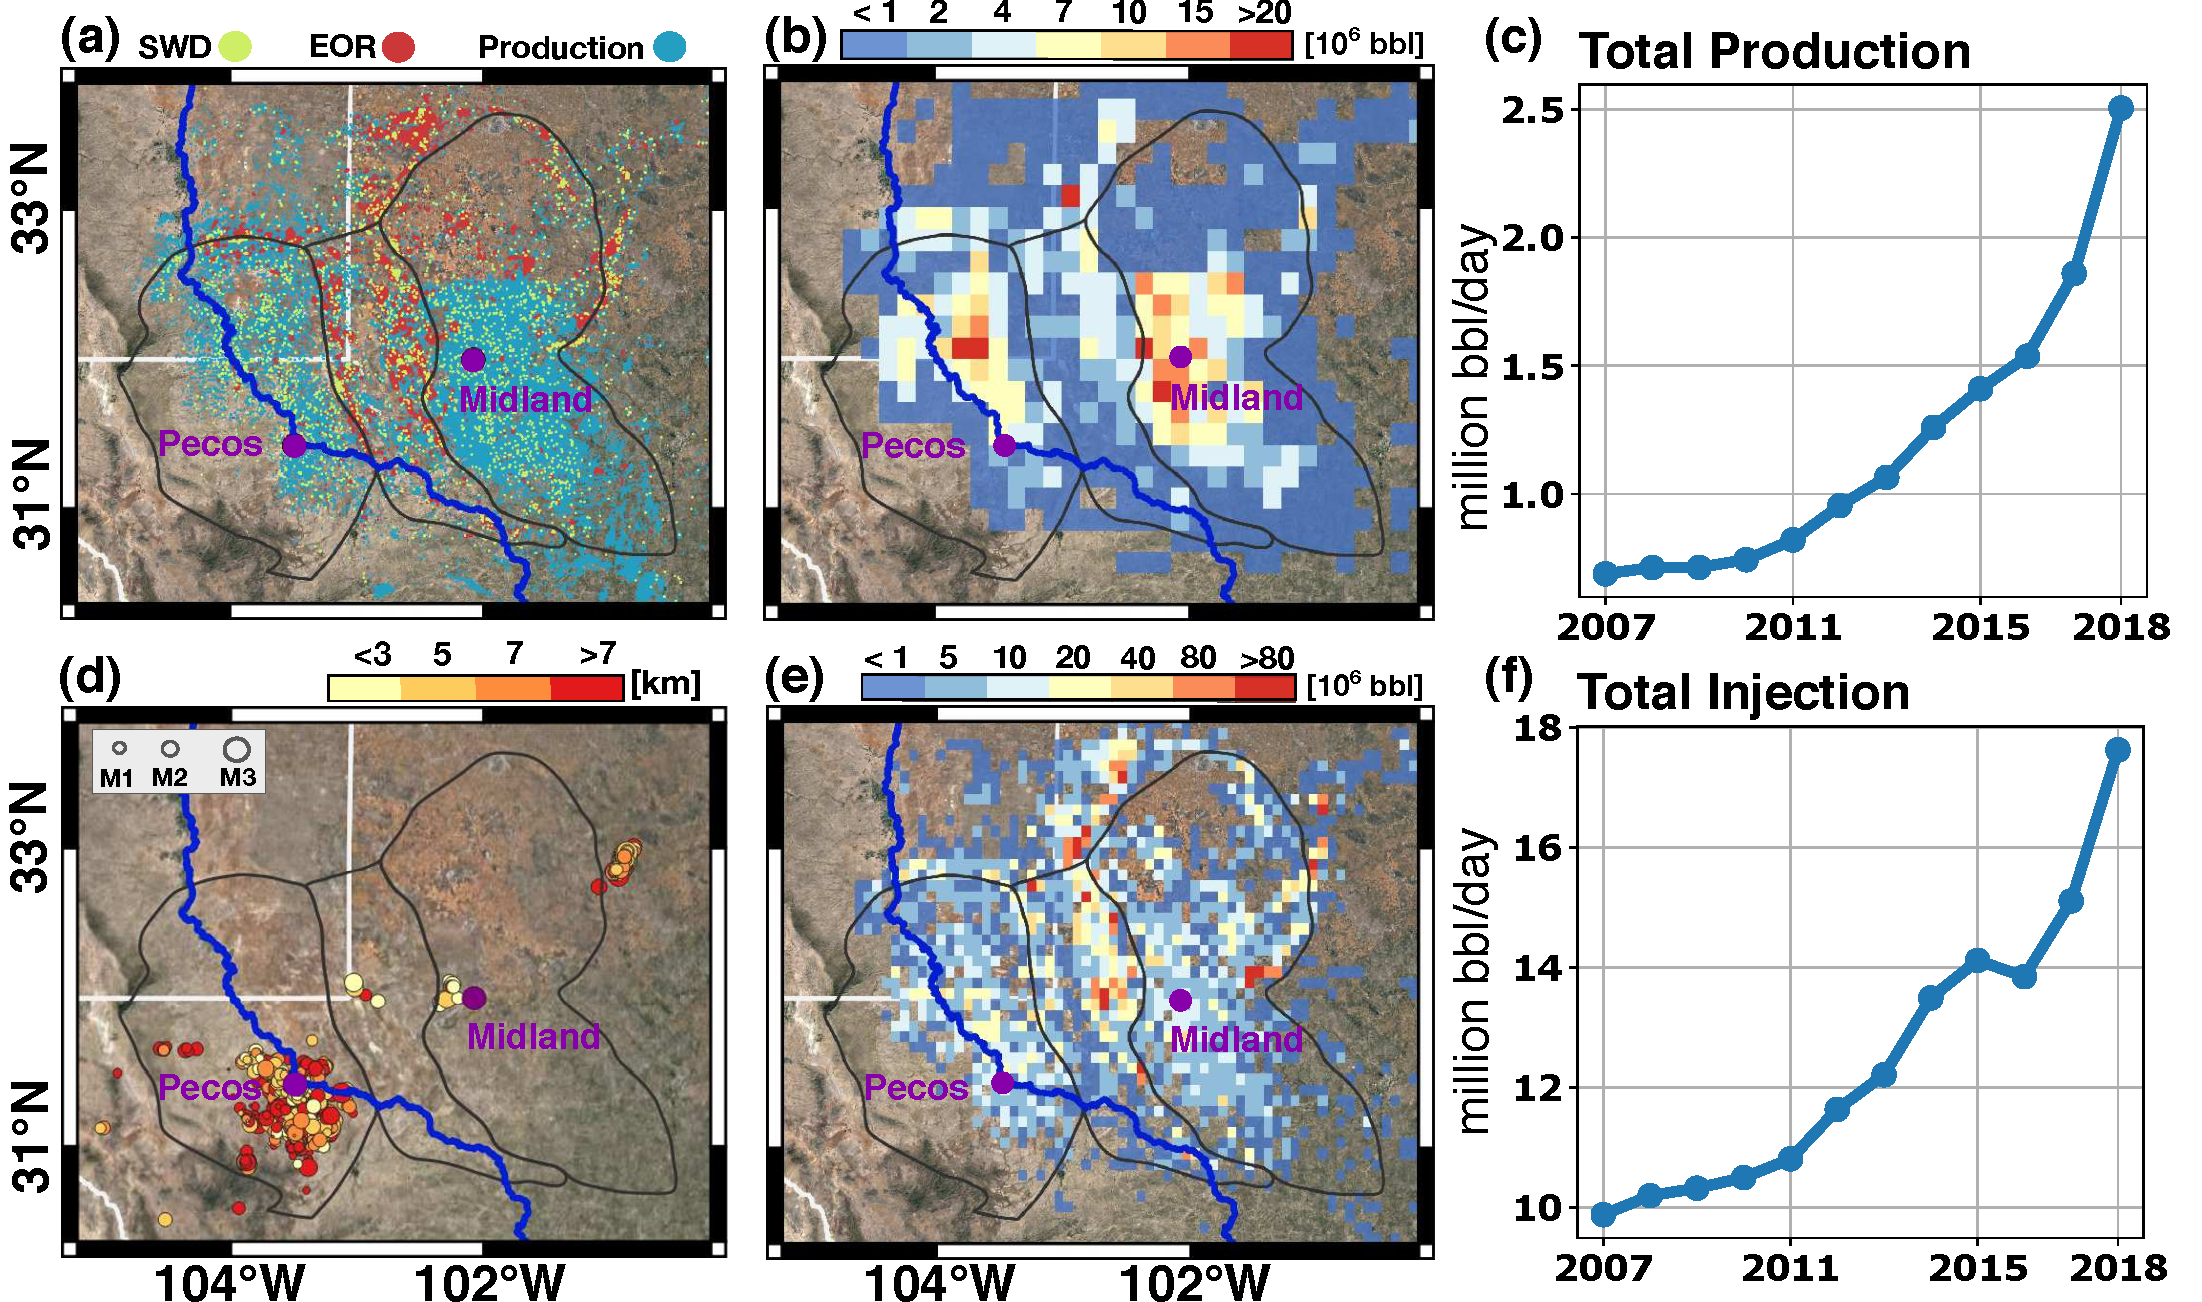
\includegraphics[width=0.99\linewidth]{figures/supplement/figureS1-cisr-data.pdf}
\caption{Shale development and induced seismicity in the Permian Basin. (a) Locations of oil production, enhanced oil recovery (EOR), and saltwater disposal (SWD) wells active in 2017. (b) Annual oil production volume on a 10-mile grid in 2017. (c) Permian region oil production rate as reported by the Texas Railroad Commission. (d) Locations of earthquake hypocenters detected by TexNet in 2017. The color and size of a circle indicates the estimated earthquake depth and magnitude. (e) Annual injection volume (including both SWD and EOR wells) on a 5-mile grid. (f) Permian region injection rate (including both SWD and EOR wells) as reported by the Texas Railroad Commission.
}
\label{fig:Permian}
\end{figure*}

Understanding the nature and causes of earthquakes and how they are linked to certain production and disposal wells requires extensive knowledge of the subsurface. InSAR surface deformation measurements allow us to estimate the distribution of fault slip at depth and infer the associated seismic risk \cite{Segall2010, huang2017fault}. Furthermore, measurements of reservoir inflation due to wastewater injection allows operators to assess pressure build-up in disposal aquifers and the associated triggered seismicity risk. It is also worth noting that oil recovery in shale wells is notoriously low \cite{clark2009determination}, and the performance of these wells varies significantly. InSAR can be employed to map subsurface fluid depletion and pressurization. These surface deformation observations, when coupled with reservoir compaction inversion modeling, can be used to assess the areal effectiveness of oil and gas extraction operations \cite{Du2001, Vasco2005}. 
echanically layered earth as a homogeneous half space, even though the stiffness increases with depth \cite{Du1992}. 


\chapter{Atmospheric Noise Analysis and Simulation}
\label{chap:atmo-noise}

This is the first line of Chapter \ref{chap:atmo-noise}, 


Ideas:

- comparison of ways people have tried to correct for troposphere

- plots/images of possible views into the single day atmosphere.
 -- modis
 -- HRRR, ECMWF
 --  GOES
 -- insar averaging
 
 axes of comparison:
 - resolution
 - time availability
 - spatial availibility
 - sensitivity to phase propation delay
 
 
 SEASONAL plots...
 
 Note

\section{Disambiguating terms from fractal surfaces, Gaussian random
fields, and power
laws}
\label{disambiguating-terms-from-fractal-surfaces-gaussian-random-fields-and-power-laws}

Part that I wanted to write down:

Another way to consider fractals: If you generate white or pink noise, unlike human speech or music, it will sound the same at any speed.

Note on Brownian motion being an integral of white noise.
For any complex sinusoid $x(t) = e^{j2 \pi f t}$ of frequency $f$, the effect in the frequency domain can found by noting that 

\begin{equation}
\int x(t) \, dt = \frac{1}{j 2 \pi f} e^{j2\pi f t} = \frac{1}{j 2 \pi f} x(t)
\end{equation}

Since integration is linear and time invariant, we can think of it as an LTI filter $h$ with frequency response $H_i(f) = \frac{1}{j 2 \pi f} $, which has a $|1/f|$ magnitude response, or $|1/f^2|$ in power.

A white noise process $w(t)$ can be defined as having a flat power spectral density (PSD) $S_W(f) = \sigma^2$. Integrating white noise results in the PSD being shaped into $S_W(f) H_i(f) = \sigma / f^2$.

\textbf{Driving question}:

Is the fractal atmospheric surface (a type of spatially correlated
noise), which has a power-law power spectrum of

\[S(f) = (1/f)^{\beta}\] also a Gaussian random field?

The three related subjects are\ldots{} - Gaussian Fields - Fractal
surfaces - Power-law power spectra Can all three be present? Or are some
mutually exclusive?

\textbf{POSSIBLE SUMMARY ANSWER}

Yes, the surface can be 1. fractal, since the structure function (aka
semi-variogram) of the atmospheric delay has a power-law form (Hanssen,
Eq 4.7.10) \footnote{Hanssen, Ramon F. Radar interferometry: data
  interpretation and error analysis. Vol. 2. Springer Science \&
  Business Media, 2001.} :

\[D_s(\rho) \sim \rho^{5/3}\]

\begin{enumerate}

\item
  A Gaussian field, since by (Cressie, 1993) Eq. 5.5.1 \footnote{Cressie,
    Noel. Statistics for spatial data. John Wiley \& Sons, 2015.},
\end{enumerate}

More generally, a fractional Brownian motion in \(R^d\) is a Gaussian
process \(Z(\cdot)\) characterized by a covariance function of the form
with

\[C(s, t) = \frac{1}{2}\left(s^{2H} + t^{2H} + |s-t|^{2H}\right)\]

and a variogram of the form

\[E[(Z(s + h) - Z(s))^2] \propto ||h||^{2H}\] So, for the Hanssen
structure fucntion, \(H=5/6\)

\begin{enumerate}
\def\labelenumi{\arabic{enumi}.}
\setcounter{enumi}{2}

\item
  A signal power law power spectrum \(S(k)\) of the form (Hanssen Eq.
  4.7.12)
\end{enumerate}

\[P(k) = P_0 \left(f/f_0\right)^{-\beta}\] where \(P_0\) is the power at
reference frequency \(f_0\) and \(\beta\) is called the \emph{spectral
index}. The structure function of a signal with this power spectrum can
be written, using the same \(\beta\), as
\[D_{\phi}(\rho) \propto \rho^{\beta-1}\] which means that if the
structure function exponent is \(5/3\), then \(\beta=8/3\) for the
spectrum slope.


(NOTE: This integral is why the vertical-line average has a slope that's 1 less than the isotropic k slope: \url{https://www.wolframalpha.com/input/?i=integral+of+1+%2F+%28x%5E2+%2B+y%5E2%29+dy+from+-c+to+c}
Start with $1 / r^2 = 1/(x^2 + y^2)$.
Then change to x/y from polar, integrate over y. it tends to 1/x for large x.

My confusion earlier: thinking that the frequency content of the signal
was doing to dictate the amplitude distribution in space (or time for
1D)\ldots{} In the same way that noise can be white (a
frequency/spectrum description) and either uniform or Gaussian (a time
or space description), the random process can be a Gaussian process, but
have the same power-law exponent.

LAST QUESTIONs: - BIGGEST UNKNOWN: Hanssen says the structure
functions/SMV is \(\rho^{5/3}\), which means in never levels off, and he
says the covariance function doesn't exist\ldots{} - Does this imply
that it can't be a Gaussian field? - \textbf{ANSWER}: most places seem
to say that fractional brownian motion is still a Gaussian field
(Brownian sheet having covariance = min(s, t)) - \textbf{TODO} This
means it has stationary increments, but isn't 2nd order
stationary\ldots{} I thought other places said ``Gaussian random fields
are 2nd order stationary (and sometimes strictly stationary under some
condition)'' - or does out limit study area + ramp removal mean in
practice it levels off\ldots{} - if a random field is Gaussian, does
it's structure func/SMV have to be gaussian?\ldots{}. NO. thats related
to the Covariance FUNCTION\ldots{} aka, the covariance of the Gaussian
variables at a given distance apart! the further away, the different the
covariance is\ldots{} but the entire process is still only characterized
by it's mean (assumed 0), and covariance function (related to the
structure function) - SO, a power-law SMV is fine for a Gaussian
process. and it will have a power law power-spectrum by FT:
https://math.stackexchange.com/questions/2173780/computing-fourier-transform-of-power-law

\begin{itemize}

\item
  I thought that Gaussian processes had have Gaussian Fourier
  transforms\ldots{}

  \begin{itemize}
  
  \item
    answer? the power spectrum relates to the FT of the covariance
    function of a (second order stationary process) (or, with different
    terms, ACF <->PSD)
  \end{itemize}
\item
  so i think ``fractal'' descriptions are orthogonal to both ``Gaussian
  process'' and ``Power spectrum'' shape\ldots{} they might just be 3
  completely separate axes, where none imply others
\end{itemize}

\hypertarget{definitions}{%
\section{Definitions}\label{definitions}}

From \cite{Hanssen2001} this, I don't see \citet{Hanssen2001} what the difference is \citep{Hanssen2001} , 4.7 intro: 

\begin{quote}
    
The behavior of atmospheric signal in radar interferograms can be mathematically described using several interrelated measures such as the power spectrum, the covariance function, the structure function, and the fractal dimension.

The power spectrum is useful to recognize scaling properties of the data or to distinguish different scaling regimes.
\end{quote}

TODO 1. Random field 1. Gaussian random field 1. Power spectrum


\subsection{Conclusions}



%% Insert the bibliography.
%% The style file, i.e., 'name.bst' for \bibliographystyle{name},
%% can be any name.bst available in your TeX distribution.
\bibliographystyle{plainnat}
\makebibliography{insar,permian,detection,imagestuff,statistics}

%% The Vita is optional, but must take no more than a single page if included.
\begin{vita}
  Full Official Name was born in Austin, Texas. After completing their work and graduating from Austin High School, they went to college somewhere, and graduated, but then decided two graduations weren't enough.
  After that, they entered the Graduate School at the University of Texas at Austin.

  %% The graduate school recommends using an email address as your address.
  \begin{address}
    scott.stanie@utexas.edu

    123 Main St.

    Austin, Texas 78712
  \end{address}

  %% declaring a typist is optional
  \declaretypist{the author}
\end{vita}

\end{document}
